\documentclass[10pt,a4paper]{article}
\usepackage{amsmath}
\usepackage{graphicx}
\usepackage{listings}

\graphicspath{{./}}

\title {9517 Project 2 Emotion Classifier}
\date {2016-10-03}
\author {Tianqi Liu\\
        \texttt{5019791}
        \and
        Hanzhang Zeng\\
        \texttt{3493047}
        }

\begin{document}
	\pagenumbering {gobble}
	\maketitle
	\newpage
	\pagenumbering {arabic}
  \section {Project and Goal}
  Our project is to do emotion recognition based on animated video or stream, we decide to recognize 4 kinds of emotions, including neutral, happy, angry and sad.

  \section {Problem Decomposition}
  the project is broken into 2 major parts, the first part is the extraction of the frontal face and the second part is training the emotional classifier. The extraction is needed because we are using fisherface to train the classifier and in order to make FisherFace work with high accuracy, the data set should have fixed size, therefore, we use Harr-cascade to extract the face. Second part is training using fisherface, which is explained in the following session.

  \section {Face Extraction}
	When we are collecting expressions from different images, we want to discard the background and other objects in the photos in order to increase the correctness of training and prediction. We use the Haar-cascade classifier. According to the Viola and Jones's object detection framework, the classifier determines the feature points by calculating the Haar-like feature by looking up to multiple rectangles (feature types) and applying the mask on the region to summarise the characteristics of the specific image.
	\begin{figure}[!ht]
  	\centering
      	
\includegraphics[width=0.3\textwidth]{Viola_Detector.png}
  	\caption{The Viola detection framework evaluates the characteristics in an image based on four kind of Haar feature}
	\end{figure}\\

	In the OpenCV implementation of Haar classifier, an improvement is made by Rainer Lienhart. Rainer took the advantages of a 45$^{\circ}$ rotation on all the Haar features
that Viola had and categorised them into four groups: Edge, Line, Centre-surround and the special diagonal line feature (Viola feature D).
	\begin{figure}[!ht]
  	\centering
      	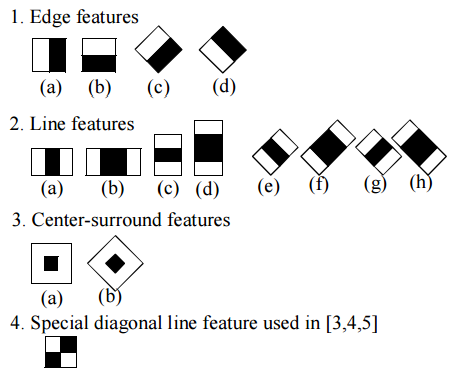
\includegraphics[width=0.4\textwidth]{Rainer_Detector.png}
  	\caption{The Rainer classifier takes advantages of rotation and enhanced line feature detections}
	\end{figure}\\

	In this project, we use frontal face cascade classifier provided by Intel Corporation. The Haar features of frontal face can be visited in OpenCV repository on GitHub.

	\section{Fisherface Recogniser}
	We use Fisherface algorithm to detect the emotion of faces. Before hand, we need to train the emotion recogniser with a large set of face images in different emotion categories (netural, angry, happy and sad). We use Cohn-Kanade database to feed our program in order to enhance its prediction accuracy.

	\section{Fisherface Recogniser Training}
	To use the Fisherface recogniser, we prepare	two sets of data, one is the training data and the other one is the test data. We feed the classifier with the training data set. The Fisherface algorithm uses LDA(Linear Discriminant Analysis) which basically downgrades the image by mapping the points to a smaller orthogonal matrix which will serve as bases for the class, such that the between class distance is maximised and the within class scatter is minimised.
  \begin{figure}[!ht]
  	\centering
      	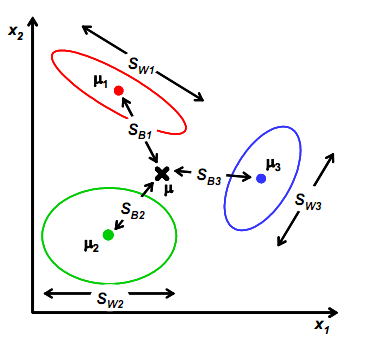
\includegraphics[width=0.3\textwidth]{fisherface.png}
  	\caption{LDA mapping}
	\end{figure}\\

  \section{Plan}
    Our plan for week11 is to implement the code for Haar-Cascade face extractor, in week12 implement the emotion classifier, and in week13 fix bugs and finalise the report.

	\begin{thebibliography}{9}
    \bibitem{Paper}
    Rainer Lienhart, Alexander Kuranov, Vadim Pisarevsky\\
    \textit{Intel Co.}\\
    Empirical Analysis of Detection Cascades of Boosted Classifiers for Rapid Object Detection

    \bibitem{Website}
    opencv.org\\
    \textit{http://docs.opencv.org/trunk/d7/d8b/tutorial\_py\_face\_detection.html}\\
    Face Detection using Haar Cascades

    \bibitem{Website}
    opencv.org\\
    \texttt{http://docs.opencv.org/2.4/modules/contrib/doc/facerec/facerec\_tutorial.html}\\
    Face Recognition with opencv
  \end{thebibliography}

\end{document}
